\documentclass[11pt,a4paper]{book}
\usepackage[utf8]{inputenc}
\usepackage[english]{babel}
\usepackage{amsmath}
\usepackage{amsfonts}
\usepackage{amssymb}
\usepackage{graphicx}
\usepackage{url}
\usepackage{python}
\usepackage{algpseudocode,algorithm}
\usepackage{tikz}
\usepackage{todonotes}


\usepackage[left=2.5cm,right=2.5cm,top=2cm,bottom=2.5cm]{geometry}

% Thesis title
%\title{Energy Efficiency, Exascale and Complex Systems}
\title{Vers l'Exascale: Des Probl\`emes Th\'eoriques aux Probl\`emes Appliqu\'es\\
The Way to Exascale: From Theorics to Applied Problems}
% Author
\author{Julien Loiseau}
% Date 
\date{\today}

\makeindex

\begin{document}


\newgeometry{left=0.5cm,right=0.5cm,top=2.0cm,bottom=1.5cm}
%% Title page -------------------------------------------------------
\thispagestyle{empty}
{%%%
%
\centering
{

\includegraphics[scale=1]{figures/style/logo_urca_front_page.jpg}
\vspace{0.5cm}
}

{
UNIVERSIT\'E DE REIMS CHAMPAGNE-ARDENNE\\
\vspace{0.5cm}
INFORMATIQUE\\
\vspace{0.5cm}
\'Ecole Doctorale Sciences Technologie Sant\'e
}

\vspace{1.0cm}
{\hrule height 2pt\vspace{2pt}}

\Large

% Title 
{\huge 
\vspace{1cm}
Hybrids Architectures to Reach Exascale
}

% Subtitle 
{
\vspace{0.5cm}
Les Architectures Hybrides pour Atteindre l'Exascale 
}

\vspace{1.0cm}
\hrule

\vspace{1.5cm}

{\LARGE
par \textbf{Julien Loiseau}
}

\vspace{2cm}

{
Th\`ese de doctorat d'Informatique
}

\vspace{2cm}

{
Sous la direction de : \textbf{M. Michaël KRAJECKI, Professeur des Universités}
}
\vspace{0.5cm}

\vspace{\fill}

{\normalsize
\begin{tabular}{l l l}
\textbf{JURY} &  & \\
&&\\
?? & ?? & Rapporteur\\
?? & ?? & Rapporteur\\
Benjamin Bergen & Docteur-Ingénieur au Los Alamos National Laboratory, USA & Examinateur \\
Guillaume Colin de Verdiere & Ingénieur au CEA, France & Examinateur\\
Michaël Krajecki & Professeur à l'Université de Reims Champagne-Ardenne & Directeur \\
François Alin & Maître de Conférences à l'Université de Reims Champagne-Ardenne & Co-directeur  \\
Christophe Jaillet & Maître de Conférences à l'Université de Reims Champagne-Ardenne & Encadrant \\

\end{tabular}

\vspace{0.5cm}

\hrule

\vspace{0.5cm}

Centre de Recherche en Sciences et Technologies de l'Information et de la Communication de l'URCA EA3804\\ 
\'Equipe Calcul et Autonomie dans les Systèmes Hétérogènes

}

%%%
}%%%
\clearpage 
\newgeometry{left=2.5cm,right=2.5cm,top=2.0cm,bottom=2.5cm}
% Empty page after title 
\thispagestyle{empty}

% Setup numbering for beginning 
\frontmatter

% Acknoledgments, thanks everybody !
\addcontentsline{toc}{chapter}{Acknowledgements}
\chapter*{Acknoledgments}

Thanks everyone ! 

\addcontentsline{toc}{chapter}{Abstract}
\hrule
\vspace{.2cm}
Titre français: \textbf{\phdTitleFR}
\vspace{.2cm}
\hrule
\vspace{.3cm}

La course à l'Exascale est entamée et tous les pays du monde rivalisent pour présenter un supercalculateur exaflopique à l'horizon 2020-2021. 
Ces superordinateurs vont servir à des fins militaires, pour montrer la puissance d'une nation, mais aussi pour des recherches sur le climat, la santé, l'automobile, physique, astrophysique et bien d'autres domaines d'application. 
Ces supercalculateurs de demain doivent respecter une enveloppe énergétique de 1 MW pour des raisons à la fois économiques et environnementales. 
Pour arriver à produire une telle machine, les architectures classiques doivent évoluer vers des machines hybrides équipées d'accélérateurs tels que les GPU, Xeon Phi, FPGA, etc. 

Nous montrons que les benchmarks actuels ne nous semblent pas suffisants pour cibler ces applications qui ont un comportement irrégulier. 
Cette étude met en place une métrique ciblant les aspects limitants des architectures de calcul: le calcul et les communications avec un comportement irrégulier. 

Le problème mettant en avant la complexité de calcul est le problème académique de Langford. 
Pour la communication nous proposons notre implémentation du benchmark du Graph500.
Ces deux métriques mettent clairement en avant l'avantage de l'utilisation d'accélérateurs, comme des GPUs, dans ces circonstances spécifiques et limitantes pour le HPC. 
Pour valider notre thèse nous proposons l'étude d'un problème réel mettant en jeu à la fois le calcul, les communications et une irrégularité extrême. 
En réalisant des simulations de physique et d'astrophysique nous montrons une nouvelle fois l'avantage de l'architecture hybride et sa scalabilité. 

\vspace{.3cm}
\hrule
\vspace{.1cm}

{
\small
Mots clés: Calcul Haute Performance, Architecture Hybrides, Simulation
}

\vspace{.1cm}
\hrule

\vspace{.4cm}
\hrule
\vspace{.2cm}
English title: \textbf{\phdTitleEN}
\vspace{.2cm}
\hrule
\vspace{.3cm}

The countries of the world are already competing for Exascale and the first exaflopics supercomputer should be release by 2020-2021.
These supercomputers will be used for military purposes, to show the power of a nation, but also for research on climate, health, physics, astrophysics and many other areas of application.
These supercomputers of tomorrow must respect an energy envelope of 1 MW for reasons both economic and environmental.
In order to create such a machine, conventional architectures must evolve to hybrid machines equipped with accelerators such as GPU, Xeon Phi, FPGA, etc.

We show that the current benchmarks do not seem sufficient to target these applications which have an irregular behavior.
This study sets up a metrics targeting the walls of computational architectures: computation and communication walls with irregular behavior.
The problem for the computational wall is the Langford's academic combinatorial problem.
We propose our implementation of the Graph500 benchmark in order to target the communication wall.

These two metrics clearly highlight the advantage of using accelerators, such as GPUs, in these specific and representative problems of HPC.
In order to validate our thesis we propose the study of a real problem bringing into play at the same time the computation, the communications and an extreme irregularity.
By performing simulations of physics and astrophysics we show once again the advantage of the hybrid architecture and its scalability.

\vspace{.3cm}
\hrule
\vspace{.1cm}

{
\small
Key works: High Performance Computing, Hybrid Architectures, Simulation
}

\vspace{.1cm}
\hrule

\vspace{.3cm}
\textbf{Discipline: \phdDiscipline}

\textbf{Spécialité: \phdSpeciality}
\vspace{.2cm}

\hspace{8cm}Université de Reims Champagne Ardenne

\hspace{8cm}Laboratoire du CReSTIC EA 3804

\hspace{8cm}UFR Sciences Exactes et Naturelles, 

\hspace{8cm}Moulin de la Housse, 51867 Reims



% Add the tableofcontentes in itself
\addcontentsline{toc}{chapter}{Contents}
\tableofcontents

% Table of figures
\addcontentsline{toc}{chapter}{List of Figures}
\listoffigures

% Table of tables
\addcontentsline{toc}{chapter}{List of Tables}
\listoftables

\mainmatter
% Introduction
\addcontentsline{toc}{chapter}{Introduction}
\chapter*{Introduction}

In the aurora 2020-2021 for United States of America and maybe before, like 2019 for China, the world of High Performance Computing (HPC) will reach another milestone in the power of machines: the Exascale. 
These supercomputers will be $100$ times faster than the estimated overfall operations performed by the human brain and its $10^{16}$ \textbf{FL}oating point \textbf{O}perations \textbf{P}er \textbf{S}econd (FLOPS) and achieve a computational power of a quintillion of ($10^{18}$) FLOPS.
This odyssey started long time ago with the first vacuum tubes computers and the need of ballistic computation for war. 
Nowadays the aim is very nearby and the power of a nation is represented by its army and money but also by the computational power of its supercomputers.
HPC's applications also spread into all the area of science and technology.\\

Since 1962, considering the Cray CDC 6600 as the first supercomputer, the power of those machines have increased following an observation of the co-fonder of the Intel company, Gordon Moore. 
Better known under the name of "Moore's Law", it speculates in 1965 that: considering the constant evolution of technology the number of transistors on a dense integrated circuit will double approximately every two years. 
Thus, the computational power, that intrinsically depends on the number of transistors on the chip, will increase; more important, as "\textit{money is the sinews of war}", the cost of the die for the same performances will decrease.  
This observation can be related to the supercomputers results through the years in the TOP500 list. 
As presented on figure~\ref{fig:intro_top500}, even if estimated in early 1965, the Moore's law seems to be accurate and sustainable. 

\begin{figure}
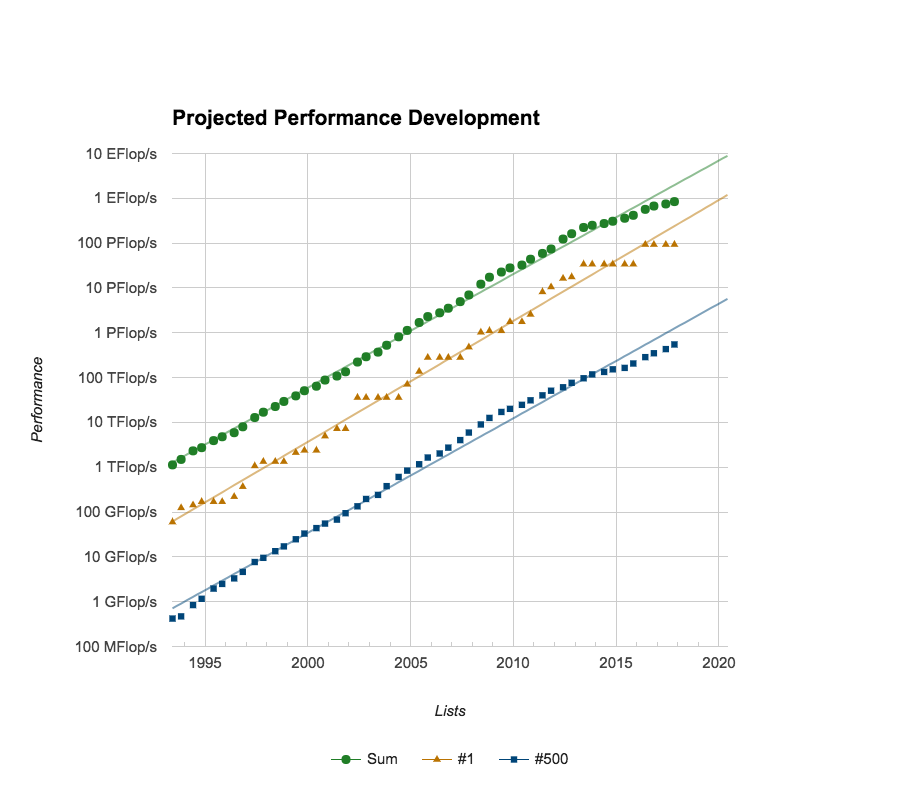
\includegraphics[width=\linewidth]{figures/introduction/top500_list_approximation.png}
\caption{Computational power evolution in the TOP500 list}
\label{fig:intro_top500}
\end{figure}

This linear evolution is not only driven by the shrink in the semiconductor with smaller transistors.
In fact the first one-core Central Processing Units (CPUs) were made using more transistors but also faster frequency.
They later faced limitations to reach high frequencies, because of the power consumption and the inherent cooling of the heat generated by the chip.
This is why, at some point in early twentieth century, IBM proposed the first multi-core processor on the same die, the Power4.
The constructors started to create chips with more than one core to increase the computational power in conjunction with the shrink of semiconductors, answering the constant demand of more powerful devices and allowing the Moore's law to thrive. 
This increase of the overall power of the chip comes with some downside costs in synchronizations steps between the cores for memory access, work sharing and complexity.
The general purpose CPU nowadays features from 2 to less than a hundred of cores on a single chip.\\

In order to reach even more computational power some researchers started to use many-core approaches. 
Using hundreds of cores these devices are using very "simple" computing units, with slow frequency and low power consumption but add more complexity and requirement for their efficient programming with even more synchronizations needed between the cores. 
Usually those many-core architectures are used coupled with a CPU that sends the data and drives them.
Some accelerators can be driven and drive regarding their configuration like the Intel Xeon Phi. 
Usually called accelerators, those devices are used in addition to the host processor to provide their efficient computational power in the key part of execution. 
The most famous accelerators are the Xeon Phi, the General Purpose Graphics Processing Unit (GPGPU) initially used in graphics, Field Programmable Gates Array (FPGA) or dedicated Application-Specific Integrated Circuit (ASIC).
The model using a host with additional device(s) appears and we will mention it as "Hybrid Architecture".
In fact a cluster can be composed of CPUs, CPUs with accelerator(s) of the same kind, CPUs with heterogeneous accelerators or even accelerators like Xeon Phi driving different kinds of accelerators.\\

Since 2013-2014 many companies, like the Gordon Moore's company \textit{Intel} itself, stated that that the Moore's law is over. 
This can be seen on figure~\ref{fig:intro_top500}: on the right part of the graph, the evolution is not linear anymore and tends to decrease slowly in time. 
This can be imputed to two main factors: on one hand, we slowly reach the maximal shrink size of the transistors implying hard to handle side effects. 
On the other hand the power wall implied by the power consumption required by so many transistors and frequency speed on the chip.

Even with all these devices, nowadays supercomputers are facing several problems in their conception and utilization. 
The three mains walls bounding the overall computational power of the machines are the power consumption wall, the communication wall and the memory wall.  
Some subproblems like the the interconnect wall, resilience wall or even the complexity wall also arise and make the task even harder.\\

In this context of doubts and questions about the future of HPC, this study propose several points of view. 
We think that the future of HPC is made with those hybrid architectures or acceleration devices adapted to the need, using well suited API, Framework and code.
We consider that the classical benchmarks, like the TOP500, are not enough to target the main walls of those architectures and especially accelerators. 
Domain scientists applications like physics/astrophysics/chemist/biologist require benchmarks based on more irregular cases with heavy computation, communications and memory accesses. 

In this document we propose a metric that extracts the three main issues of HPC and apply them to accelerated architectures to figure out how to take advantage of those architectures and what the limitations are. 
The first step to this metrics is obtained when merging two characteristic problems and then a third one combining all our knowledge.
The first two are targeting computation and communication wall over very irregular cases with high memory accesses, using an academic combinatorial problem and the Graph500 benchmark. 
The last is a computational scientific problem that covers both difficulties of the previous problems and appears to be hard to implement on supercomputers and even more on accelerated ones.\\

This thesis is composed of 3 parts.

The first develop the state of the art in HPC from the main laws to the hardware. 	
We go through the basic laws from Amdahl's to Gustafson's laws and the specification of speedup and efficiency.
Classical CPUs, GPGPUs and other accelerators are described and discussed regarding the state of the art. 
The main methods of ranking and the issues regarding them are presented.\\ 

In the second part we propose our metric based on characteristic problems to target classical and hybrid architectures.
The Langford problem is described as an irregular and computationally heavy problem.
This shows how the accelerators, in this case GPUs, are able to support the memory and computation wall. 
This allowed us to beat a world record with the last instances of this academic problem.
The Graph500 problem is then proposed as an irregular and communications heavy problem. 
We present our implementation, and more over the logic to take advantage of the GPUs computational power for realistic applications. \\

In the third part we consider a problem that is heavy and irregular regarding to computation and communications.
We analyze it and show that it combine all the previous limitations. 
Then we apply our methodology and show how nowadays supercomputers can overcome those issues. 
This computational science problem is based on the Smoothed Particle Hydrodynamics method.
Based on our global work to efficiently parallelize those kind of production application, we intend to provide an efficient tool for physicists and astrophysicists called FleCSPH. 
The former application we started with was developed on top of the FleCSI framework from the Los Alamos National Laboratory it allowed us to exchange directly with the LANL domain scientists on their need.\\

The last part will conclude on this work and results and show some of the main prospects of this study and my future researches. 
% Chapter One
\chapter{HPC and Exascale}


\section{Introduction}

The HPC world is spread over all the scientific domains nowaday and is used from usual computation to the biggest black holes merging simulations. 
Firstly, we present the rules, laws and organization that characterize the HPC world from the Moore's law, Amdhal with the Flynn Taxonomy and the description of the recent bottlenecks and walls. 

Considering homogeneous cluster only. 

\section{Parallelism}



\subsection{Flynn taxonomy}

The flynn taxonomy presents a hierarchical organization of computation machine.

In this classification \cite{flynn1972some}, Michael J. Flynn present the SIMD,SISI, MISD and MIMD.
Add table and present some example of machines

\subsection{Goals}

\subsubsection{Speedup}

Speedup can be separate in two parts, Latency and Throughput.

\subsection{Bottlenecks}

\subsection{Amdahl and Gustafson}

The Amdahl's\cite{amdahl1967validity} law is use to find the theoretical speedup in latency of a program.
We can separate a program in two parts, the one that can be execute in parallel and the one that is sequential. 
And even if we reduce the parallel part to infinite the sequential part will reach 100\% of the total time. 

Extracted from the Amdahl paper the law can be writen as: 

\begin{equation}
Speedup = \frac{1}{Seq + \frac{Par}{n}}
\end{equation}

Where $Seq + Par = 1$ and $Seq$ and $Par$ respectively the sequential and parallel ratio of a program. 

On plot XXX, a representation of the perfect speedup is represented.
This law does not take every cases in acount. 
Indeed the speedup can be much better if we grow the amount of work to be done in the same time as the number of processes that execute the program. 

This is proposed by the Gustafson law presented in. 

\section{Hardware}

The structure of an HPC cluster can be 

\subsection{Classical CPU}

\subsection{GPU}

\subsection{FPGA and ASICS}

\section{Clusters and Exascale}

\subsection{Benchmarking}

\subsubsection{TOP500}

The TOP500 list is a list of the 500 most powerful super computers in the world.
The ranking is based on the LINPACK and LAPACK suite. 
Initialy the LINPACK, Linear Algebra library was used but is now replaced by the new Linear Algreba Pack, LAPACK. 

\subsection{Composition and usage}

\subsection{Interconnection}

\section{Languages}

\subsection{Accelerators}

\subsection{Runtimes}

\section{Optimization}


\subsubsection{Memory locality}

\subsubsection{Vectorization}

\subsection{CPU specifications}

\subsection{GPUs specifications}

\subsection{Communications}

\section{Conclusion}

% Chapter Two 
\chapter{Complex systems}

\section{Introduction}

\section{Combinatorial problems}

\subsection{Combinatorial search}

\subsection{Combinatorial optimization}

\section{A case study, the Langford problem}

Use the articles here for figures and a base report. 
 
\section{Complex systems as a benchmark} 

\section{GRAPH500}

Use the articles here too 
 
\section{Conclusion}
% Chapter Three 
\part{Application}

\chapter{Physics and Astrophysics}

\section{Fluids}
\section{Binary Neutron Stars}

\chapter{FleCSPH}

\section{FleCSI}
\section{FleCSPH applications}
% Conclusion
\addcontentsline{toc}{chapter}{Conclusion}
\chapter*{Conclusion}

% Annexes
`\addcontentsline{toc}{chapter}{Annexes}
\chapter*{Annexes}


% Bibliography
\addcontentsline{toc}{chapter}{Bibliography}
\bibliographystyle{alpha}
\nocite{*}
\bibliography{biblio/biblio_langford,biblio/biblio_graph,biblio/biblio_sph,biblio/biblio_hpc}

\end{document}
